\documentclass[FIPLY_base.tex]{subfiles}

\author{Andreas Denkmayr}
\date{20. Dezember 2015}

\begin{document}
\section{Fragments}
\subsection{Was sind Fragments?}
Ein Fragment stellt einen Teil der Benutzeroberfläche einer Activity zur Verfügung, dabei kann man mehrere Fragments in einer Activity verwenden und diese zur Laufzeit auswechseln.
Da Fragments in mehreren Activities wiederverwendet werden können, müssen Ansichten wie Detailviews oder Listen nur einmal programmiert werden und können überall eingesetzt werden.
Fragments werden ab Android 3.0 (API level 11) zur Verfügung gestellt. \newline
Bei der Implementierung von Fragments wurde die Dokumentation zu diesen [\citetitle{adFragments} \cite{adFragments}] und der jeweilige Developer Guide [\citetitle{adFragmentsGuide} \cite{adFragmentsGuide}] verwendet. 

\begin{figure}[h]
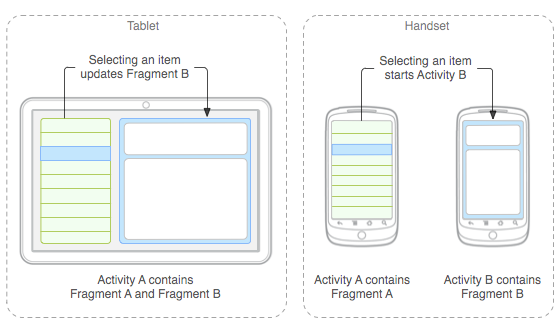
\includegraphics[scale=0.60]{img/fragments_modules}
\caption{Beispiel man kann mithilfe von Fragments Views erstellen, die sowohl auf einem Tablet als auch auf einem Handy ein optimales Benutzerinterface anbieten. [\citetitle{adFragmentsGuide} \cite{adFragmentsGuide}]}
\end{figure}

\newpage
\subsection{Der Lifecycle}
Ein Fragment ist immer eingebunden in eine Activity und ist direkt vom Lifecycle der übergeordneten Activity abhängig.
Wird die übergeordnete Activity pausiert oder zerstört werden auch alle zugeordneten Fragments pausiert oder zerstört.
\ \\
\begin{lstlisting}
@Override
public View onCreateView(LayoutInflater inflater, ViewGroup container, Bundle savedInstanceState) {
        super.onCreate(savedInstanceState);
        return inflater.inflate(R.layout.exampleFragment, container, false);
    }
\end{lstlisting}
Das Aufbauen der Benutzeransicht erfolgt in der onCreateView() Methode eines Fragments. In diesem Fall wird das layout XML file exampleFragment angezeigt.
\subsection{Fragment Transactions}
Mittels Transaktionen lassen sich Fragments hinzufügen, entfernen oder ersetzen.
Es werden mehrere dieser Aktionen hintereinander abgesetzt und zusammen nach einem commit() ausgeführt.
Ein Fragment kann mittels addToBackStack() auch zum BackStack hinzugefügt werden um dadurch, ähnlich wie bei Activites, Navigation mit dem BackButton zu ermöglichen.
Dabei ist zu beachten, dass alle Aktionen vor einem commit() gemeinsam auf den BackStack gelegt werden und bei drücken des BackButtons alle gemeinsam aufgehoben werden.
Wird addToBackStack() nicht aufgerufen, wird ein Fragment beim Schließen oder beim Wechseln auf ein anderes Fragment zerstört und kann nicht mehr aufgerufen werden.

\begin{lstlisting}
Fragment exampleFragment = new ExampleFragment();
FragmentManager fragmentManager = getFragmentManager();
FragmentTransaction fragmentTransaction = fragmentManager
	.beginTransaction();
fragmentTransaction.addToBackStack(null);
fragmentTransaction.replace(R.id.fraPlace, exampleFragment);
fragmentTransaction.commit();
\end{lstlisting}
Hier wird ein ExampleFragment erstellt, man ersetzt das Fragment das sich aktuell im FrameLayout R.id.fraPlace befindet mit dem erstellten exampleFragment und fügt es zum Backstack hinzu.


\newpage
\subsection{Verwendung von Fragments}
In dieser Arbeit werden Fragments verwendet, um die Benutzeransichten, ausgenommen des NavigationDrawers, anzuzeigen.
Dabei wird ein FrameLayout im Layoutfile der MainActivity durch ein Fragment mittels der displayView() Methode ersetzt.
Navigation durch diese Fragments wird mittels den Buttons im FMain oder dem NavigationDrawer ermöglicht.
Zusätzlich werden verschachtelte Fragments verwendet um komplexere Ansichten darzustellen. In diesem Fall wird in den layout XML files der Fragments ein FrameLayout erstellte und die verschachtelten Fragments werden dann in diesen neuen FrameLayouts angezeigt.
\ \\
\begin{lstlisting}
private void displayView(Fragment fragment) {
        FragmentManager fragmentManager = getFragmentManager();
        FragmentTransaction fragmentTransaction = fragmentManager
        	.beginTransaction();
        fragmentTransaction.addToBackStack(null);
        fragmentTransaction.replace(R.id.fraPlace, fragment);
        fragmentTransaction.commit();
    }
\end{lstlisting}
Methoden wie diese werden immer wieder verwendet um die Fragment Transactions an einem Ort zusammenzufassen und den Code so lesbarer zu machen.

\ \\
\begin{lstlisting}
<FrameLayout
        android:id="@+id/fraPlace"
        android:layout_width="match_parent"
        android:layout_height="match_parent" />
\end{lstlisting}
So sieht ein FrameLayout aus das wir immer wieder verwenden, um darin Fragments anzuzeigen.

\newpage
\begin{figure}[t] % Bilder aktualisieren
	\begin{subfigure}[h]{0.3\textwidth}
	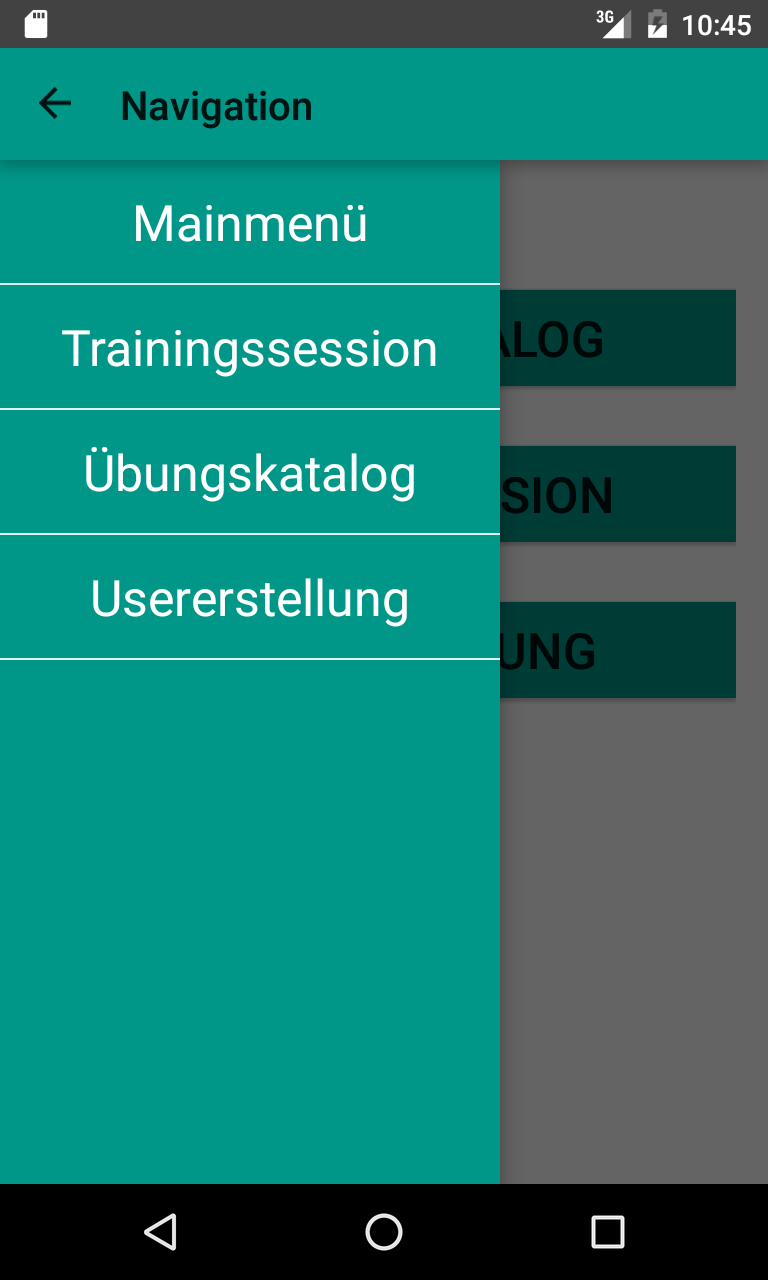
\includegraphics[scale=0.20]{img/NavigationDrawer}
	\end{subfigure}
	\hfil
	\begin{subfigure}[h]{0.3\textwidth}
	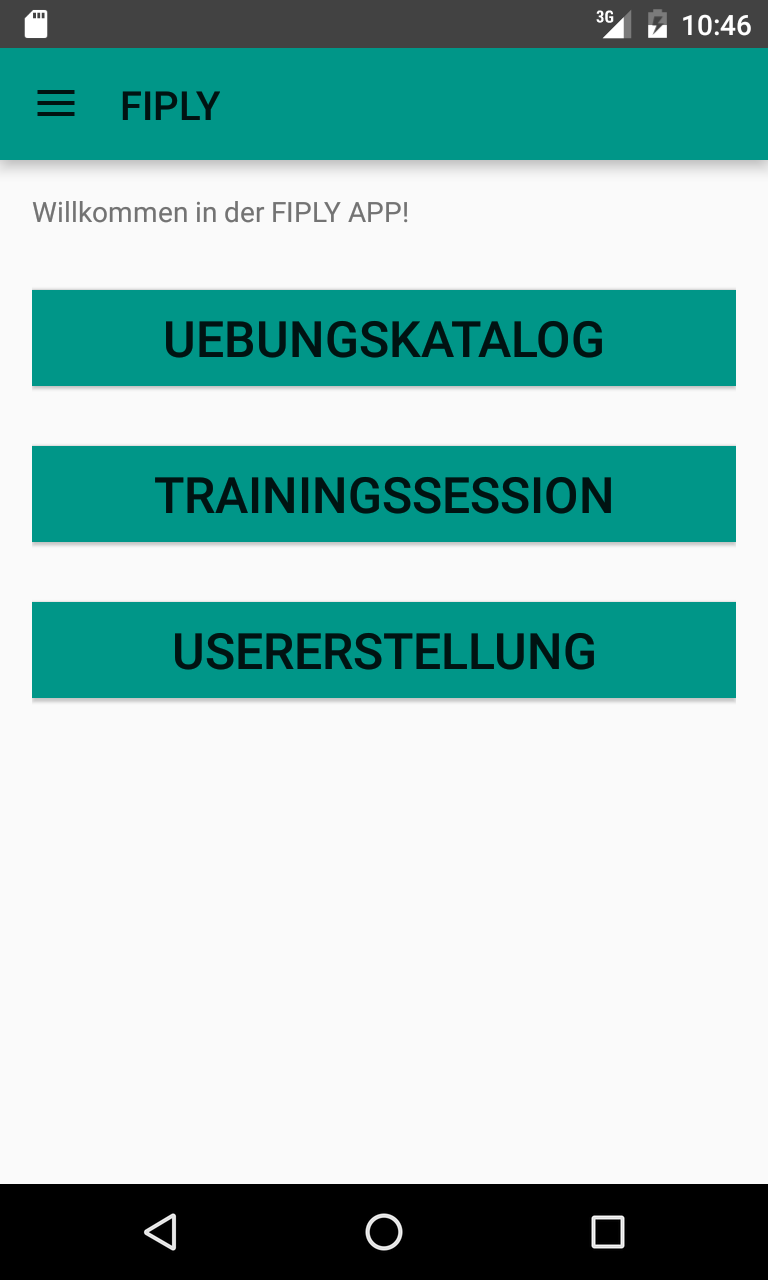
\includegraphics[scale=0.20]{img/MFragment}
	\end{subfigure}	
	\caption{Bild des NavigationDrawers und des FMains} 
	\ \\
	\begin{subfigure}[h]{0.3\textwidth}
	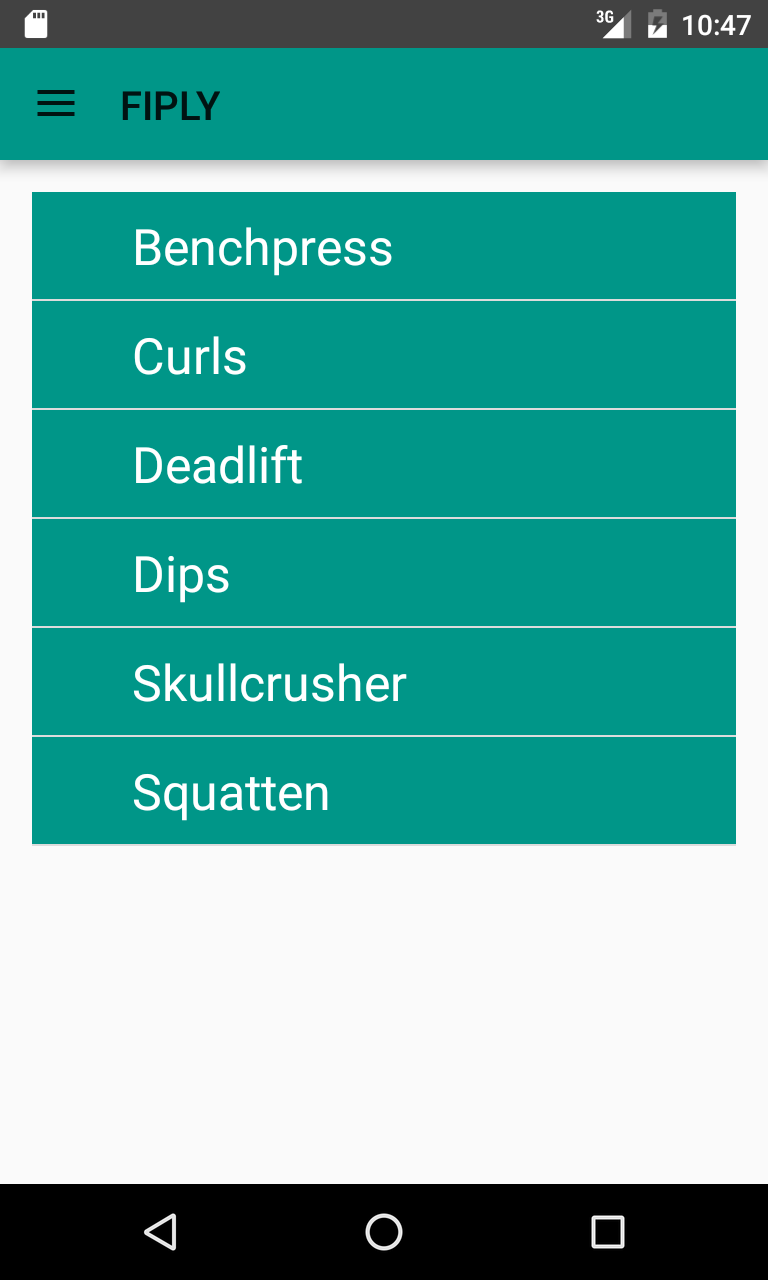
\includegraphics[scale=0.20]{img/Uebungskatalog}
	\end{subfigure}
	\hfil
	\begin{subfigure}[h]{0.3\textwidth}
	
\includegraphics[scale=0.20]{img/Uebungskatalog_detail_video}
	\end{subfigure}	
	\caption{Bei Klicken eines Elements in der ListView wird die zugehörige DetailView aufgerufen}
\end{figure}

\end{document}
